\documentclass[11pt]{article}
\usepackage[margin=1in]{geometry}
\usepackage{amsmath,amsthm,amssymb}
\usepackage{enumitem, graphicx, float, caption}
\usepackage{amsmath}
\usepackage{bm}
\usepackage{parskip}
\usepackage{lipsum}
\usepackage{tikz}
\usepackage{listings}
\usepackage{xcolor}
\usepackage{colortbl}
\usepackage{float}
\usepackage{subcaption}
\usepackage{graphicx}
\usepackage[utf8]{inputenc}
\usetikzlibrary{arrows.meta}

\definecolor{codegreen}{rgb}{0,0.6,0}
\definecolor{codegray}{rgb}{0.5,0.5,0.5}
\definecolor{codepurple}{rgb}{0.58,0,0.82}
\definecolor{backcolour}{rgb}{0.95,0.95,0.92}

\lstdefinestyle{mystyle}{
    backgroundcolor=\color{backcolour},
    commentstyle=\color{codegreen},
    keywordstyle=\color{magenta},
    numberstyle=\tiny\color{codegray},
    stringstyle=\color{codepurple},
    basicstyle=\ttfamily\tiny,
    breakatwhitespace=false,
    breaklines=true,
    captionpos=b,
    keepspaces=true,
    numbers=left,
    numbersep=5pt,
    showspaces=false,
    showstringspaces=false,
    showtabs=false,
    tabsize=2
}

\lstset{xleftmargin=.020\textwidth, xrightmargin=.020\textwidth}

\setcounter{MaxMatrixCols}{26}
\setlength\parindent{0pt}
\counterwithin{equation}{enumi}


\begin{document}
    \noindent Nathan Burwig \\
    Math 87 HW 7 \\
    Due 11/12/2022
    
    \hrulefill
    
    \section{The Germinator}

    Suppose we are monitoring a population of bacteria in a lab. Initially there 
    are 500 organisms. You’ve predicted that everyday the population grows by 
    6.35\%. Furthermore, suppose that you introduce an additional m organisms 
    to the population everyday.

    \begin{enumerate}
        \item \textbf{Write a recurrence relation for the population after $k$ 
            days, $p_k$, as a function of $p_{k-1}$ and $m$.}

            We know that we have an initial population of 500, and that number
            will grow every day based on the percentage growth of $6.35\%$ and
            that we also have some random number of $m$ additional organisms
            joining per day. Thus we can describe the population growth in
            general by...
            \[
                p_k = 1.0635p_{k-1} + m
            \] 
        \item \textbf{Solve this recurrence relation for $p_k$ as a function of $m$ 
            and $k$ (i.e. no explicit reference to $p_{k-1}$).}

            Generally a good method to go about solving these kinds of problems
            are to just write out the first few terms of the serires and
            attempt to notice a pattern. Inductive proofs can be handy but are
            oftentimes overkill. Let's see if we can find something here...
            \begin{align*}
                p_0 &= 500 \\
                p_1 &= 1.0635p_0 + m \\
                p_2 &= 1.0635p_1 + m = 1.0635^2 p_0 + 1.0635m + m \\
                p_3 &= 1.0635^3 p_0 + 1.0635^2 m + 1.0635m + m 
            \end{align*}
            It is here we notice a pattern emerge, and we can extrapolate to
            determine what this would look like for general $k$.
            \[
                p_k = 1.0635^kp_0 + (1.0635^{k-1} + 1.0635^{k-2} + \cdots + 1)m
            \] 
            The parenthetical section is a geometric seires, thus we can sum it
            using the summation equation for a geometric series. It would then
            become...
            \[
                -\frac{m(1-1.0635^k)}{0.0635} 
            \] 
            We then have the general form for $p_k$ to be...
            \[
                p_k = 1.0635^k \cdot {500} - \frac{m(1-1.0635^k)}{0.0635} 
            \] 
            \newpage
        \item \textbf{Suppose that you are breeding the bacteria for an experiment, 
            and need a fixed number of organisms g. Find an expression for the 
            day, k, in which your desired number of organisms g, as a function of m.}
            
            What we want is to say there is some desired number of organism,
            and what day $k$ will give us that desired amount. If we set our
            equation $p_k$ equal to the desired number $g$, then we can solve
            it for $k$. A highlight of the algebra goes as follows.
            \begin{align*}
                g &= 1.0635^k \cdot {500} - \frac{m(1-1.0635^k)}{0.0635} \\
                0.0635g + m &= 1.0635^k(500 \cdot 0.0635 + m) \\
                \ln{\left[ \frac{0.0635 + m}{31.75 + m} \right]} &= k \ln{\left[ 1.0635 \right]} \\
                k &= \frac{\ln{\left[ 0.0635 + m \right]} - \ln{\left[ 31.75 + m \right]}}
                          {\ln{\left[ 1.0635 \right]}} 
            \end{align*}
            And that is our expression for day $k$
        \item \textbf{Write a python function that takes in goal population g 
            and the added amount of organisms m, and returns the number of days, 
            k, to reach the goal. Suppose the goal balance is 200,000 organisms. 
            How many days does it take to reach the goal if we introduce 100 
            bacteria a day? 250? How many months does it take to reach a goal of 
            2,000,000 introducing 100 and 250?}

            We can quickly write a ptyhon function to check these values.
            Taking $m = 100$ with a goal population of $200,000$, it would take
            75 days. If $m=250$ with the same goal, then it takes only $63$
            days. 

            Evaluating how many months it would take to reach $2,000,000$
            organisms is a similar process, however this time we divide the
            number of days by the average length of the month, or about $30$
            days. For $m = 100$ we get $3.7$ months, and if we gained $250$ per
            day it would only take $3.3$ months.
    \end{enumerate}

    \section{How effective is regression?}

    In this exercise, we investigate the quality of a linear least squares
    regression as a function of the amount of noise in our data.


    \begin{enumerate}
        \item \textbf{Consider a linear equation $y = mx + b$. Precisely explain 
            how one could randomly sample points satisfying this equation, under 
            the constraints that the samples $0 \leq x \leq N$ for some $N$. Suppose you then 
            performed least linear squares regression on the data. With enough 
            samples, you should be able to recover the equation of the line. What 
            is the minimum number of samples needed in order to do this?}

            In general, we could utilize the \texttt{random} function from
            \texttt{python} to randomly generate some numbers. Then, given the
            constraint that each point is on the line given by some $m$ and
            $b$, we would have points on the line.

            We would generate those points by saying something along the lines
            of \texttt{x = random.randint(0, N)}. This would produce numbers
            randomly, and, if we got two of these points, that would be enough
            to reproduce the equation of the line.
        \item \textbf{Suppose that we have introduced some noise to our equation, 
            i.e. our samples are drawn from $y = mx+ b+ \eta$, where $\eta$ is drawn 
            from a normal distribution with mean $0$ and variance $\sigma$. One would
            hope that, with enough samples, one could recover the equation of 
            the original line. Predict how $\sigma$ affects the number of samples 
            required to approximate the line.}

            We know that our variance will affect the width of the distribution
            of points we generate. If we have a set of points with a wider
            distribution, then we will need to sample more points the average
            out to the actual equation of the line. If our $\sigma$ is smaller,
            then we will need fewer points in order to reproduce the equation
            of the line.

        \item \textbf{For concreteness, let $m = 3,b = 4,M = 10$. Sample and plot 
            (on separate plots) 100 points sampled from $y = mx + b + \eta$ for 
            $\sigma = 0.01,0.1,1,5,30$ and plot the original (i.e. no noise) 
            line over the data.} 

            We can utilize \texttt{matplotlib} to help us plot these lines and
            label them based on the variance we use.

            \begin{minipage}[t]{0.48\linewidth}
                \begin{center}
                    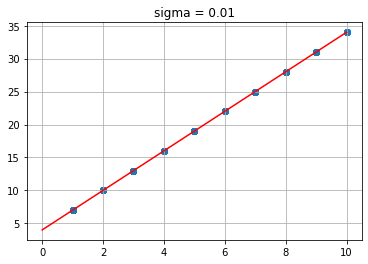
\includegraphics[width=\linewidth]{s.01.png}
                    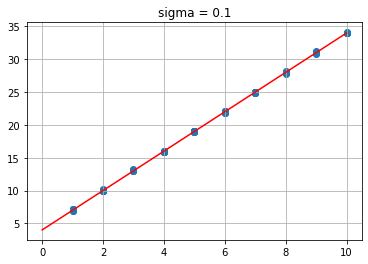
\includegraphics[width=\linewidth]{s.1.png}
                \end{center}
            \end{minipage}\hfill\vline\hfill%
            \begin{minipage}[t]{0.48\linewidth}
                \begin{center}
                    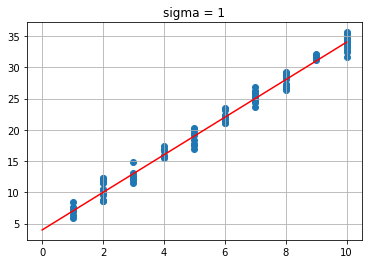
\includegraphics[width=\linewidth]{s1.png}
                    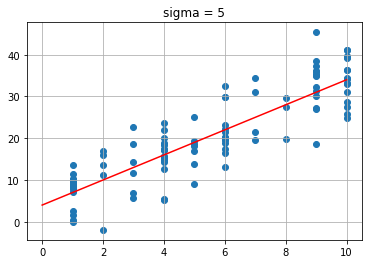
\includegraphics[width=\linewidth]{s5.png}
                \end{center}
            \end{minipage}
            \begin{center}
                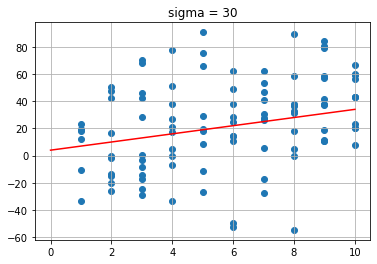
\includegraphics[width=0.54\linewidth]{s30.png}
            \end{center}
            This is a fairly expected outcome.
        \item \textbf{Perform least linear squares on the data obtained in the 
            preceding part. The solution will give you the coefficients of a 
            line. On each plot, plot this line over the data.}

            We can perform least squares regression quite easily using the
            \texttt{polyfit} module of \texttt{matplotlib.pyplot}. We can also
            code this manually, and for completness, I went ahead and did a
            couple out on paper to make sure I was getting numbers that were
            accurate to the plots given by polyfit. The results are given
            below.

            \begin{minipage}[t]{0.48\linewidth}
                \begin{center}
                    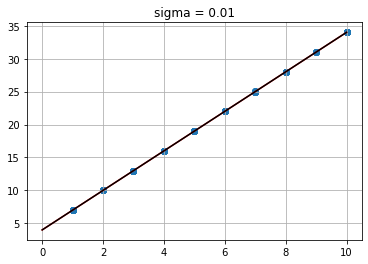
\includegraphics[width=\linewidth]{sr.01.png}
                    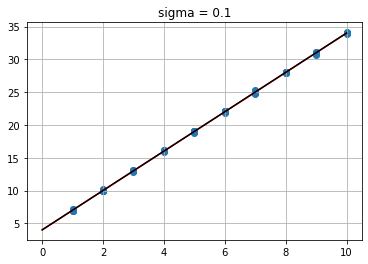
\includegraphics[width=\linewidth]{sr.1.png}
                \end{center}
            \end{minipage}\hfill\vline\hfill%
            \begin{minipage}[t]{0.48\linewidth}
                \begin{center}
                    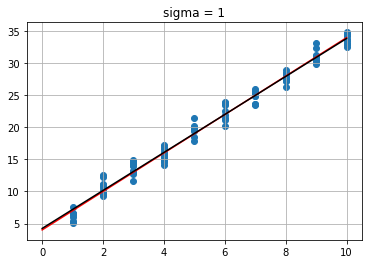
\includegraphics[width=\linewidth]{sr1.png}
                    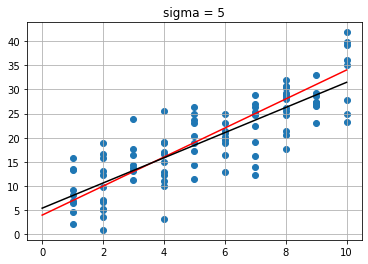
\includegraphics[width=\linewidth]{sr5.png}
                \end{center}
            \end{minipage}
            \begin{center}
                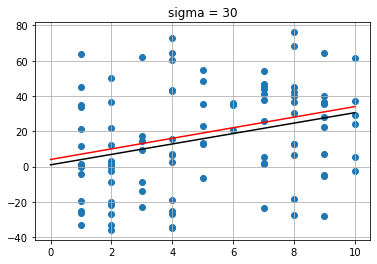
\includegraphics[width=0.54\linewidth]{sr30.png}
            \end{center}
            We can see that it is just as we expected. The accuracy to the
            actual line is determined by the variance in our data, and as we
            increase that variance, we get farther away from represting the
            original line.
        \item \textbf{Run an experiment to determine how many samples are needed in order 
            for the least squares solution to be within 0.01 of the coefficients 
            of the original line for each value of $\sigma$ (you do not need to find the
            minimal such value, just some number of samples that works). For each 
            value of $\sigma$, plot the error in slope (i.e. the difference between the 
            slope of the original line and the one computed by least squares
            regression) for the following number of samples:
            $20,200,2000,20000,200000$.}

            We can determine the error and plot them in a table based on the
            given sigma and sample size. I found the error by just using the
            standard error formula based on the actual slow ($m=3$) and the
            slope obtained during the regression. The table plots as follows...

            \begin{center}
                \begin{tabular}{||c||c|c|c|c|c||}
                    \hline
                    \multicolumn{6}{||c||}{Error} \\
                    \hline
                    \hline
                    --	&	0.01	&	0.1	&	1	&	5	&	30 \\
                    \hline\hline
                    20	    &	\cellcolor{green}0.00051 	& \cellcolor{green}0.00493  & 0.06094    &	0.09329    & 4.49227\\
                    200	    &	9.270e-05	&	0.00041  & 0.05218    &	0.21477    & 0.75302\\
                    2000	&	1.897e-05	&	0.00032  & \cellcolor{green}0.00352    &	0.03483    & 0.16247 \\
                    20000	&	8.058e-07	&	0.00016  & 0.00428    & \cellcolor{green}0.00875    & 0.06850\\
                    200000	&	5.410e-06	&	1.620e-05& 0.00100	  &	0.00433 & \cellcolor{green}0.007773 \\
                    \hline
                \end{tabular}
            \end{center}
            I've gone ahead and marked the cells which pass the 0.01 criteria
            in green. Across the top row is the variance, and the left most
            column is the sample size.

            This confirms our previous thoughts, showing that the wider the
            variance, the more samples we need in order to get a smaller error
            between the two lines. 
    \end{enumerate}

\end{document}

